Integrating an interpreter in \chef requires preparing a virtual machine that includes the interpreter binary, a symbolic test library, and a launcher.
%
To communicate with the interpreter runtime, \chef provides an API (Table~\ref{tab:chef:api}) that will be explained along with its use.

\begin{table}
\centering
\small
\begin{tabular}{| l | l | }
\hline
\textbf{API Call} & \textbf{Description} \\
\hline
\codebit{log\_pc(pc, opcode)} & Log the interpreter PC and opcode \\
\hline
\codebit{start\_symbolic()} & Start the symbolic execution \\
\codebit{end\_symbolic()} & Terminate the symbolic state \\
\hline
\codebit{make\_symbolic(buf)} & Make buffer symbolic \\
\codebit{concretize(buf)} & Concretize buffer of bytes \\
\codebit{upper\_bound(value)} & Get maximum value for expression on current path \\
\codebit{is\_symbolic(buf)} & Check if buffer is symbolic \\
\codebit{assume(expr)} & Assume constraint \\
\hline
\end{tabular}
\caption{The \chef API used by the interpreters running inside the S2E VM.}
\label{tab:chef:api}
\end{table}

\paragraph{Preparing the Interpreter Binary}

In principle, \chef can run unmodified interpreters for major popular languages, such as Python and JavaScript.
%
\chef automatically obtains from the running interpreter the stream of high-level program counters (HLPCs) for each execution path, required by the state adapter to reconstruct the high-level symbolic execution tree (Section~\ref{sec:chef:hlcf}).

In practice, however, applying a number of optimizations in the interpreter implementation significantly improve symbolic execution performance (Section~\ref{sec:chef:optimizeforsymbex}).


\paragraph{The Symbolic Test Library}

The unit of symbolic execution in \chef is the \emph{symbolic test}.
%
A symbolic test is a class, function, or other language-specific construct that encapsulates the symbolic input setup, the invocation, and the property checking of the feature targeted by the test.
%
A symbolic test is similar to a unit test, except for an extra set of primitives for creating symbolic values.

The symbolic tests are written in the same language as the target, and require runtime support in the form of a language-specific \emph{symbolic test library}.
%
The symbolic test library provides the developer interface for writing symbolic tests.
%
In addition, it translates the requests for marking language values as symbolic into the \chef API primitives for marking memory buffers as symbolic (the \codebit{make\_symbolic} call, together with the \codebit{assume} call for defining conditions over the input).
%
For example, when a symbolic test requests a 10-character symbolic string, the symbolic test library creates a concrete 10-character string object, then it finds its buffer address in the internal representation and marks the buffer as symbolic.
%
As a result, the symbolic test library is typically implemented as a native extension module, so it gains access to the internal data structures of the interpreter.

%% During symbolic execution, the low-level engine generates test cases as concrete assignments to the memory bytes marked as symbolic.
%% %
%% The \chef test library takes care of translating the concrete bytes back to string objects reported as test cases to the developer.

The execution of the interpreter in the virtual machine is bootstrapped by a launcher.  The launcher receives the location of the symbolic test (e.g., the module file and the class name, for Python) and runs the interpreter binary with the appropriate arguments such that it starts executing the symbolic test.
%
The launcher is typically a small web server running inside the guest, listening for commands from \chef.

%%%%%%%%%%%%%%%%%%%%%%%%%%%%%%%%%%%%%%%%%%%%%%%%%%%%%%%%%%%%%%%%%%%%%%%%%%%%%%%%

\subsection{Automated High-level Control Flow Detection in Interpreters}
\label{sec:chef:hlcf}

We defined a high-level path as a sequence of statements identified by high-level program counters (HLPCs).  In this section, we present the concrete semantics of the HLPC and how \chef obtains it automatically from a running interpreter.

\begin{figure}
  \centering
  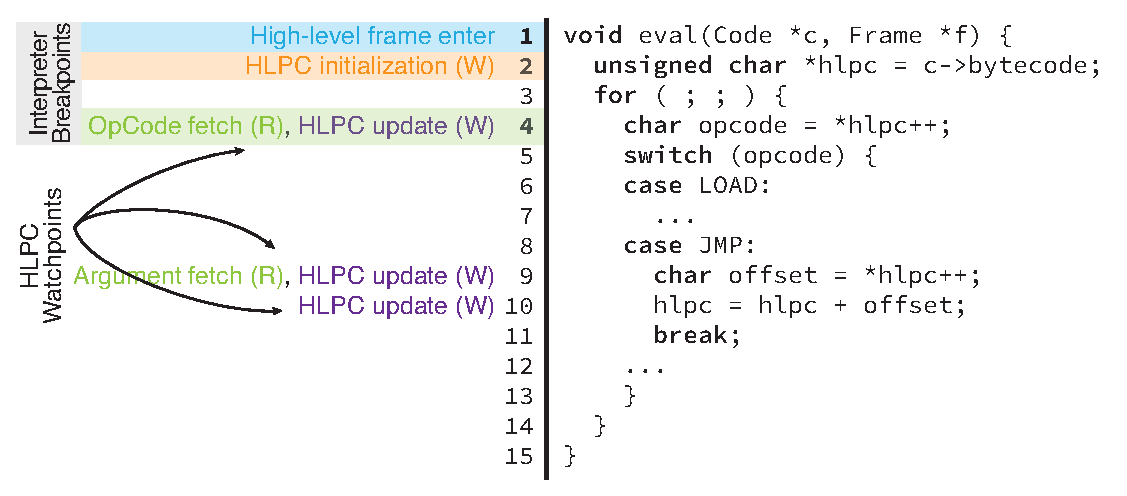
\includegraphics[width=0.8\textwidth]{chef/figures/interp-model}
  \caption{Structure of interpretation loop in most common interpreters.  Lines 1, 2, and 4 are three key HLPC points.  High-level control flow changes at Lines 4, 9, and 10 are detected at runtime by watchpoints on HLPC address identified at Line 2.}
  \label{fig:chef:interp-model}
\end{figure}

\paragraph{Standard Interpretation Model}

In general, obtaining the high-level program counter in a running interpreter is undecidable, because the boundaries between program statements are a high-level property of the language, and the separation may not reflect in the low-level implementation.
%
Even at the high level, statement boundaries may be ambiguous due to functional constructs, such as lambda functions and list comprehensions, or data definitions mixed with control flow, such as the class definitions in Python.

In practice, however, most interpreters follow a common structure that \emph{can be detected automatically}.
%
Instead of directly interpreting the source program, interpreters first compile it to an intermediate bytecode representation, which is interpreted instruction by instruction.  The bytecode is typically kept in per-function memory buffers.
%
When a function is called, the interpreter pushes a frame on its high-level stack, which contains a pointer variable to the next instruction in the function bytecode buffer.
%
An interpretation function receives the function bytecode and the stack frame, then executes the bytecode instructions one by one, while updating the HLPC variable of the frame (the right half of Figure~\ref{fig:chef:interp-model}).
%
We confirmed the generality of this approach by inspecting the source code of the most popular interpreters for Python, JavaScript (Mozilla's SpiderMonkey and WebKit's JavaScriptCore), Ruby, PHP, and Lua.

For these interpreters, we define the \chef high-level statements to be bytecode instructions, and their HLPC to be their address in the bytecode buffer.
%
As a result, to track the HLPC of the execution state, \chef monitors updates to the HLPC variable of the top high-level stack frame.

\paragraph{Tracking the HLPC Variable in the Interpreter}

To obtain the address of the top HLPC variable on the stack, \chef monitors three key locations in the interpretation function that summarize its HLPC update behavior:
%
(1) the address of the function itself, (2) the address of the statement that initializes the HLPC variable, and (3) the address of the statement that fetches the next opcode in the bytecode buffer.  The locations are highlighted on the left half of Figure~\ref{fig:chef:interp-model}.
%
\chef uses them as follows.

First, \chef maintains a stack of HLPC frames that track the interpreter's own high-level frames.
%
When the interpreter enters the interpretation function, \chef pushes a new HLPC frame on the current execution state.  A HLPC frame contains the address of the HLPC variable and its last value in the corresponding high-level frame of the interpreter.

Second, when the interpreter executes the HLPC initialization statement, \chef stores in the HLPC frame the memory address written to by the statement as the address of the HLPC variable.

Third, when the interpreter executes the opcode fetching statement, \chef marks the beginning of a new high-level statement at the address given by the current HLPC value.

During the execution of the interpretation function, \chef sets a watchpoint on the HLPC variable in the current frame.
%
When the variable is updated---e.g., when the next instruction is fetched, or after a branch or loop iteration---\chef correspondingly updates the HLPC value and the high-level symbolic execution tree, as needed.

\paragraph{Constructing the Interpreter HLPC Summary}

Before an interpreter is used for symbolic execution, \chef constructs its three-location HLPC summary.
%
The summary is constructed once for each interpreter binary.

First, \chef records all memory writes in the interpreter, when running a special developer-provided ``calibration'' script.
%
For each write, \chef records the interpreter location (x86 PC), the memory address, and the value written.

The role of the calibration script is to create HLPC update patterns that are recognizable among other memory writes.
%
The calibration script should run long enough that the HLPC patterns become clearly distinguishable.

To this end, \chef uses a linear sequence of instructions to create a linear HLPC update pattern.
%
We assume that the interpreter compiles a linear program (no branches) to a linear sequence of bytecode instructions.

After all memory writes are collected, \chef groups them by address and discards the groups whose values are not monotonically increasing.
%
Among the remaining groups, \chef discards those with fewer writes than the number of statements in the calibration program.  For this step, we assume that each statement corresponds to one or more bytecode instructions.
%
Finally, \chef discrads the groups whose write value deltas are larger than the size of a bytecode instruction.  We empirically determined an upper bound threshold of 1KB.

At the end, there should be exactly one remaining group, whose address refers to the HLPC variable of the frame of the recorded execution.

From the HLPC variable, \chef obtains the three-location summary.
%
The HLPC initialization location is the x86 PC of the first write operation in the remaining group.
%
The HLPC initialization location then leads to the address of the interpretation function, either by dynamically tracking the low-level program stack, or by using debug symbols in the interpreter binary.
%
Finally, the opcode fetch point corresponds to the first memory read of the HLPC variable, inside the interpretation function.

In case the calibration ends with no remaining memory write group, or more than one group remaining, the calibration fails.
%
This could happen, for instance, when the calibration is attempted on a non-conforming interpreter, or when the calibration script is too short.  To this end, we empirically determined that a 100-statement calibration script is sufficient for a successful calibration for all interpreters we tested.

In principle, defining program statements at an intermediate representation risks missing paths at the high-level.
%
This would happen, for instance, if the interpreter translated code with complex control flow to a linear bytecode sequence.
%
However, in our experience, we noticed that the translated bytecode follows closely the structure of the program.
%
In particular, interpreters perform little or no optimization on the bytecode.

\paragraph{Manually Annotating the High-level Program Counter}

When the interpreter structure diverges from our assumptions, \chef provides a fallback option of manually annotating the interpreter with the HLPC information.


%%%%%%%%%%%%%%%%%%%%%%%%%%%%%%%%%%%%%%%%%%%%%%%%%%%%%%%%%%%%%%%%%%%%%%%%%%%%%%%%

\subsection{Interpreter Optimizations}
\label{sec:chef:optimizeforsymbex}

In order to maximize performance, interpreters make heavy use of special cases and sophisticated data structures.  Unfortunately, these features hurt the performance of symbolic execution by amplifying path explosion and increasing the complexity of symbolic formulas~\cite{overify}.

We identify a number of optimizations that preserve the interpretation semantics but significantly improve symbolic execution performance.  The optimizations use the \chef API in the last block of rows in Table~\ref{tab:chef:api}.

\paragraph{Neutralizing Hash Functions}

Hash functions are especially common in interpreters, due to the internal use of hash tables for associative data structures (e.g., Python dictionaries or Lua tables).  However, they are generally a problem in symbolic execution: a symbolic value added to a hash table (a)~creates constraints that essentially ask the constraint solver to reverse a hash function, which is often hard, and (b)~causes the exploration to fork on each possible hash bucket the value could fall into.
%
A simple and effective optimization is to \emph{neutralize the hash function}, i.e., replace it with a degenerate one returning a single constant. This change honors the usual contracts for hash functions (equal objects have equal hashes) and will turn hash lookups into list traversals.

\paragraph{Avoiding Symbolic Pointers}

Input-dependent pointers (also referred to as symbolic pointers) may point to multiple locations in the program memory, so a pointer dereference operation would have to be resolved for each possible location.  In practice, symbolic execution engines deal with this situation in one of two ways:
%
(a)~fork the execution state for each possible concrete value the symbolic pointer can take; or
%
(b)~represent the dereference symbolically as a read operation from memory at a symbolic offset and let the constraint solver ``deal'' with it.
%
Both ways hurt symbolic execution, either by causing excessive path explosion or by burdening the constraint solver.

While there is no generic way to avoid symbolic pointers other than concretizing their values (the \codebit{concretize} API call) at the price of losing completeness, there are specific cases where they can be avoided.

First, \emph{the size of a buffer can be concretized} before allocation.  A symbolic size would most likely cause a symbolic pointer to be returned, since a memory allocator computes the location of a new block based on the requested size.  To avoid losing completeness, a symbolic execution-aware memory allocator can determine a (concrete) upper bound on the requested size and use that value for reserving space, while leaving the original size variable symbolic.  This way, memory accesses to the allocated block would not risk being out of bounds.  Figure~\ref{fig:sym-malloc} shows how the \chef API is used to wrap a call to the \codebit{malloc} function in the standard C library.

\begin{figure}
  \centering
  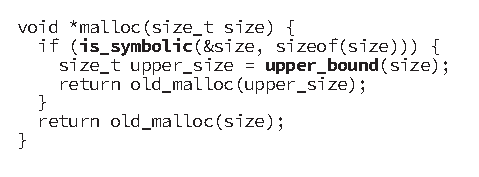
\includegraphics[width=2.6in]{chef/figures/mallocopt}
  \caption{Example of a symbolic execution-aware \codebit{malloc} function wrapper created using the \chef API.  If the allocation size is symbolic, the wrapper determines its upper bound and issues a concrete request to the underlying implementation.}
  \label{fig:sym-malloc}
\end{figure}

Second, \emph{caching and ``interning'' can be eliminated}.  Caching computed results and value interning (i.e., ensuring that a single copy of each possible value of a type is created) are common ways to improve the performance of interpreters.  Alas, when a particular value is computed, its location in memory becomes dependent on its value. If the value was already in the cache or in the interned store, it is returned from there, otherwise a new value is computed.  During symbolic execution, this logic becomes embedded in the value of the returned pointer, which becomes symbolic.  Disabling caching and interning may hurt the native performance of the program, but it can give a significant boost when running inside a symbolic execution engine.

\paragraph{Avoiding Fast Paths}

A common way to speed-up the native performance of a function is to handle different classes of inputs using faster specialized implementations (``fast paths'').  For example, a string comparison automatically returns false if the two strings have different lengths, without resorting to byte-wise comparison.

Fast paths may hurt symbolic execution because they cause symbolic branches in the code checking for the special input conditions.  \emph{Eliminating short-circuited returns} can reduce path explosion.  Instead of returning to the caller as soon as it produced an answer, the function continues running and stops on an input-independent condition.  For example, when comparing two strings of concrete length, a byte-wise string comparison would then traverse the entire string buffers in a single execution path, instead of returning after the first difference found.


%%% Local Variables: 
%%% mode: latex
%%% eval: (visual-line-mode)
%%% fill-column: 1000000
%%% TeX-master: "main"
%%% End:
